\chapter{Example process}
\label{chp:airsep}

    To investigate optimization techniques an example process to which they can be applied is needed.
    The cryogenic air separation process serves well as a demonstrative case. This process is highly 
    complex due to a high degree of material and energy integration as well as extreme operating conditions. 
    
    This chapters first aims at providing some background on different air separation technologies, which are 
    discussed in the first section. Afterwards a concrete process flowsheet, which will be referred to in the 
    remainder of this thesis, is introduced and examined. 
    
    \section{Air separation technology}
    \begin{figure}[h]
    	\begingroup%
  \makeatletter%
    \setlength{\unitlength}{1cm}%
  \makeatother%
  \begin{picture}(17, 7)%	
    \scriptsize
    \put(2,1){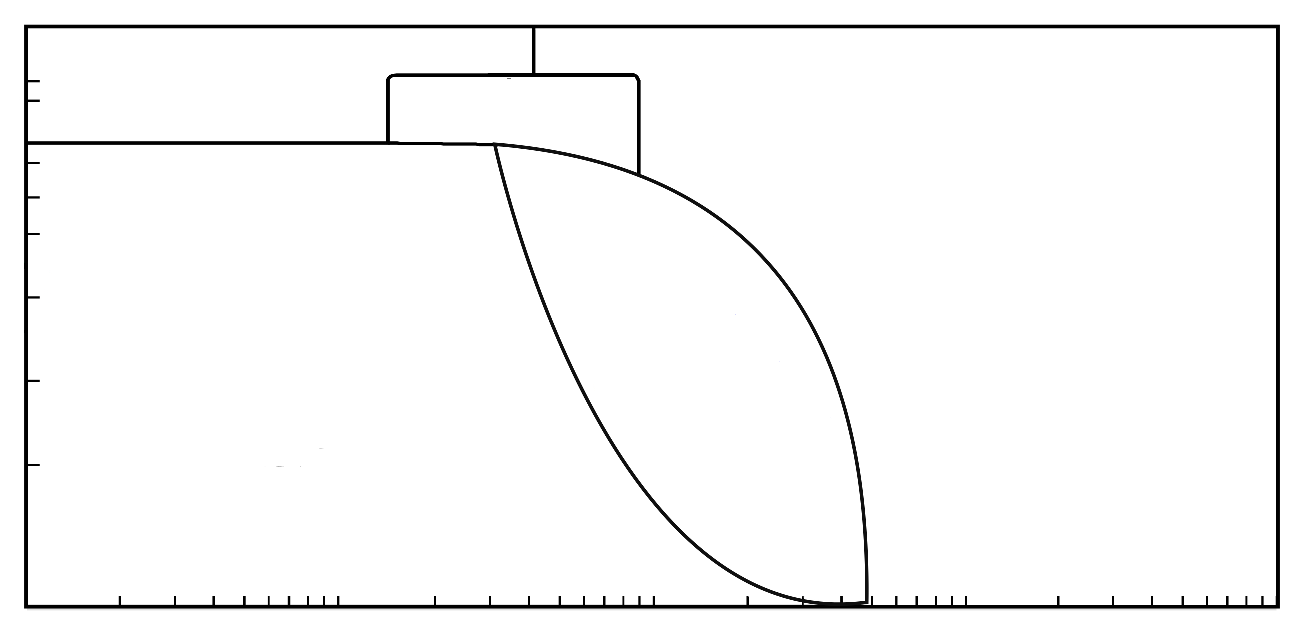
\includegraphics[width=13cm]{Pictures/tech_comp_graph.eps}}%
    \put(8.5, 0.1){\color[rgb]{0,0,0}\makebox(0,0)[c]{\smash{\normalsize{product stream $[\frac{m^3_{STP}}{h}]$}}}}%
    \put(0.6, 4){\color[rgb]{0,0,0}\rotatebox{90}{\makebox(0,0)[c]{\smash{\normalsize{$N_2$-purity $x_{N_2, Ret}$ $[\%]$}}}}}%
    \put(1.9, 0.65){\color[rgb]{0,0,0}\makebox(0,0)[l]{\smash{$10$}}}%
    \put(5.15, 0.65){\color[rgb]{0,0,0}\makebox(0,0)[l]{\smash{$10^2$}}}%
    \put(8.35, 0.65){\color[rgb]{0,0,0}\makebox(0,0)[l]{\smash{$10^3$}}}%
    \put(11.55, 0.65){\color[rgb]{0,0,0}\makebox(0,0)[l]{\smash{$10^4$}}}%
    \put(14.75, 0.65){\color[rgb]{0,0,0}\makebox(0,0)[l]{\smash{$10^5$}}}%
    \put(1.85, 1){\color[rgb]{0,0,0}\makebox(0,0)[r]{\smash{$95$}}}%
    \put(1.85, 2.45){\color[rgb]{0,0,0}\makebox(0,0)[r]{\smash{$97$}}}%
    \put(1.85, 3.325){\color[rgb]{0,0,0}\makebox(0,0)[r]{\smash{$98$}}}%
    \put(1.85, 4.15){\color[rgb]{0,0,0}\makebox(0,0)[r]{\smash{$99$}}}%
    \put(1.85, 4.8){\color[rgb]{0,0,0}\makebox(0,0)[r]{\smash{$99.5$}}}%
    \put(1.85, 5.2){\color[rgb]{0,0,0}\makebox(0,0)[r]{\smash{$99.9$}}}%
    \put(1.85, 5.55){\color[rgb]{0,0,0}\makebox(0,0)[r]{\smash{$99.95$}}}%
    \put(1.85, 6.1){\color[rgb]{0,0,0}\makebox(0,0)[r]{\smash{$99.99$}}}%
    \put(1.85, 6.4){\color[rgb]{0,0,0}\makebox(0,0)[r]{\smash{$99.999$}}}%
    \put(1.85, 6.4){\color[rgb]{0,0,0}\makebox(0,0)[r]{\smash{}}}%
    \put(5,3){\color[rgb]{0,0,0}\normalsize{\CM{membrane processes / \\ gas permeation}}}%
    \put(8.9,3.7){\color[rgb]{0,0,0}\normalsize{\CM{PSA}}}%
    \put(7,6.20){\color[rgb]{0,0,0}\scriptsize{\CM{membrane \& \\ post oxidation}}}%
    \put(4,6.5){\color[rgb]{0,0,0}\normalsize{\CM{cryogenic processes \\ (liquid)}}}%
    \put(12,5.5){\color[rgb]{0,0,0}\normalsize{\CM{cryogenic processes \\ (gaseous)}}}%
  \end{picture}%
\endgroup%

    	\caption{Comparison of Air Separation Technologies \cite{Prasad.1994}.}
    	\label{fig:tech_compar}
    \end{figure}
    The separation of air finds many application in the modern industry. Pure oxygen and nitrogen are
    are essential for many processes. The yearly amount of oxygen extracted from air exceeds 100 million
    tonnes and nitrogen even surpassing these numbers \cite{Emsley.2003c2001}. Among the most prominent
    examples is the production of synthesis gas,
    which forms the basis for a multitude of very large-scale process operations. In addition the
    air separation processes find application as a utility provider rather than producer
    for example in highly efficient integrated combustion cycles \cite{Mahapatra.2010}. Due to the
    many different applications, pure nitrogen or oxygen is needed with various demands on
    purity, flow rate or phase composition. Therefore different technologies are suitable to specific tasks.

    In general three main principles of air separation can be identified; adsorption,
    cryogenic distillation and transport through membranes. \Figref{fig:tech_compar} illustrates the
    economically most viable processes depending on product stream volume and purity.
    In the further course of this chapter the most prevalent  air separation technologies
    along with their main fields of application and economic scope are introduced.

        \subsection{Cryogenic processes}
        \label{sec:cryo_air_sep}

        \begin{figure}
            \center
            \begin{tikzpicture}
    \pgfmathsetmacro{\blockh}{1.5cm}
    \pgfmathsetmacro{\blockw}{2.2cm}
    \tikzset{box/.style={draw, rectangle, minimum height=\blockh, minimum width=\blockw, align=center}}
    \node (A) [box] at (0,0) {air \\ compression} ;
    \node (B) [box] at ($(A) + (0,-3)$) {air pre- \\ treatment} ;
    \draw [arrow] (A.south) -- (B.north) ;
    \node (C) [box] at ($(B) + (4,0)$) {heat \\ exchange} ;
    \draw [arrow] ($(B.east) - (0,0.5)$) -- ($(C.west) - (0,0.5)$) ;
    \node (D) [box] at ($(B) + (8,0)$) {cryogenic \\ separation} ;
    \node (E) [box] at ($(B) + (12,0)$) {storage} ;
    \node (F) [box] at ($(A) + (8,0)$) {product \\ compression} ;
    \node (G) [box] at ($(A) + (12,0)$) {product \\ delivery} ;
    \draw [arrow] ($(C.east) - (0,0.5)$) -- ($(D.west) - (0,0.5)$) ;
    \draw [arrow] ($(D.west) + (0,0.5)$) -- ($(C.east) + (0,0.5)$) ;
    \draw [arrow] (D.west) -- (C.east) ;
    \draw [arrow] (D.east) -- (E.west) ;
    \draw [arrow] ($(E.north) + (0.5,0)$) -- ($(G.south) + (0.5,0)$) ;
    \draw [arrow] ($(C.west) + (0,0.5)$) -- ++(-0.5,0) -- ++(0,1) -- (11.5,-1.5) -- ($(G.south) - (0.5,0)$) ;
    \draw [arrow] (C.west) -- ++(-1,0) -- ++(0,3) -- (F.west) ;
    \draw [arrow] (F.east) -- (G.west) ;
\end{tikzpicture}

            \caption[Air Separation Unit]{Schematic representation of the cryogenic air separation process.}
            \label{fig:ASU}
        \end{figure}
        Cryogenic air separation processes are implemented over a great variety of industries among others refining,
        petrochemicals, medical, food \& beverages and environmental \cite{Sirdeshpande.2005}. \Figref{fig:ASU}
        shows the major unit operations associated with the process. Initially the air is compressed and later re-expanded
        to reach the low temperatures required for liquefaction. In an intermediate pre-treatment step most unwanted
        contaminants are removed. Particularly the amount of carbon dioxide in the gas carries great significance, as
        operating conditions lie beneath its freezing point. Due to freeze out at those low temperatures, especially
        within the heat exchanger the performance of process units can greatly be reduced, or entirely hindered.
        The pre-treated air is then cooled against product streams leaving the separation stage of the process. To which extend
        the refrigeration is  recovered is among the most dominant factors for economic operations. The requirements
        towards the product streams determine how much can be recovered. Most processes produce gaseous streams at
        approximately ambient pressure and temperature \cite{Smith.2001} and hence recover the maximum of energy from the
        process. However often a subsequent compression step or even liquefaction step is employed to deliver the
        desired product to the consumer.

        In terms of economically feasible operations, the compression denotes a sizable contribution to the capital cost
        and is responsible for the majority of the operating cost. However when recovering liquid product, the
        compression work needs to increase in order to compensate for the loss in recoverable refrigeration. Due to the widespread
        application of the  process, several increasingly complex process configurations are being implemented
        with different strategies, for internal recovery of pressure energy and refrigeration.

        The cryogenic process can most economically simultaneously produce large quantities of highly pure oxygen and nitrogen.
        In addition argon and other noble gases can be recovered from the process. Most alternative technologies will
        produce one single product stream. Additionally the economy of scale can very well be exploited for this
        process, which is why current developments are towards large scale single train that can produce
        an excess of several thousand tonnes of product stream per day \cite{Castle.2002}.

        \subsection{Adsorption processes}
        \label{sec:psa}
        Certain materials display a higher affinity to adsorb a specific class of molecules. Nitrogen is
        more easily adsorbed in zeolites than oxygen. Therefore if air is fed through a
        zeolite bed, an oxygen rich stream is produced. Since any bed will eventually
        be saturated and its capability for adsorption be exhausted, the process carries an
        inherent discontinuity. However, for most processes which yield large product streams,
        continuous operations are more cost effective.

        To realize a continuous process multiple adsorption vessels are operated simultaneously.
        Once a bed is saturated, the process is switched to a different vessel and the saturated one
        is regenerated. Regeneration utilizes the change of adsorption capabilities at varying temperature
        or pressure. By increasing temperature or lowering pressure can the bed therefore be regenerated.
        Due to the switching during operations these processes a commonly known as Temperature Swing Adsorption
        (TSA) or Pressure Swing Adsorption (PSA). For most industrial applications PSA is preferred for its
        simpler operation and faster cycle times \cite{Smith.2001}.

        The ability to construct very compact units, have led to implementations of PSA processes at
        very different scales. Briefcase sized units are constructed for treatment of asthma patients or other
        medical appliances. Larger scale plants have successfully been utilized, for example in the paper industry
        during the de-lignation of pulp \cite{Nelson.1993}.

        The bed size is the determining factor for equipment cost. Since cycle times are limited by the regeneration
        step, the bed size and therefore the cost increases rapidly with the product flowrate. For very large
        scale operations the cryogenic process is more economically viable. However the PSA/TSA process can be operated
        much more flexible due to drastically shorter start-up times compared to the cryogenic process. Furthermore, no
        by-products can be recovered from the process without further subsequent separations \cite{Choi.2003}.

        \begin{figure}
        	\center
        	
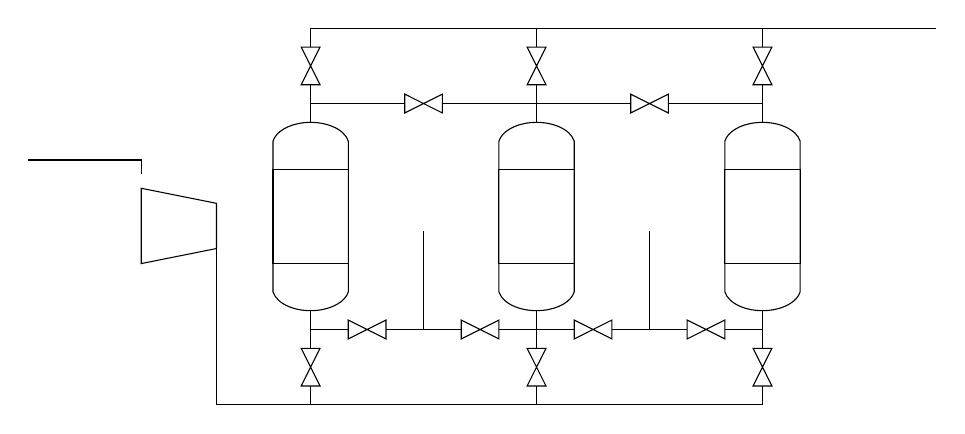
\begin{tikzpicture}[y=0.80pt,x=0.80pt,yscale=-1, inner sep=0pt, outer sep=0pt]
  \begin{scope}[shift={(331.654,-501.732)}]
      \path[draw](0.0000,833.3900){[rotate=-180.0] arc(349.729:190.271:17.287000 and
        10.358)} -- (34.0200,765.3500){[rotate=-180.0] arc(169.729:10.271:17.287000
        and 10.358)} -- (0.0000,833.3900) -- cycle;
      \path[draw,rounded corners=0.0000cm] (0.0000,778.1100) rectangle (34.0157,820.6297);
  \end{scope}
  \begin{scope}[shift={(433.701,-501.732)}]
      \path[draw](0.0000,833.3900){[rotate=-180.0] arc(349.729:190.271:17.287000 and
        10.358)} -- (34.0200,765.3500){[rotate=-180.0] arc(169.729:10.271:17.287000
        and 10.358)} -- (0.0000,833.3900) -- cycle;
      \path[draw,rounded corners=0.0000cm] (0.0000,778.1100) rectangle (34.0157,820.6297);
  \end{scope}
  \begin{scope}[shift={(535.748,-501.732)}]
      \path[draw](0.0000,833.3900){[rotate=-180.0] arc(349.729:190.271:17.287000 and
        10.358)} -- (34.0200,765.3500){[rotate=-180.0] arc(169.729:10.271:17.287000
        and 10.358)} -- (0.0000,833.3900) -- cycle;
      \path[draw,rounded corners=0.0000cm] (0.0000,778.1100) rectangle (34.0157,820.6297);
  \end{scope}
  \begin{scope}[shift={(272.126,-522.992)}]
    \path[draw](0.0000,841.8900) -- (34.0200,835.0900) -- (34.0200,814.6800) --
      (0.0000,807.8700) -- (0.0000,841.8900) -- cycle;
  \end{scope}
  \begin{scope}[shift={(1182.05,357.165)},rotate=90.0]
    \path[draw](0.0000,829.1300) -- (0.0000,837.6400) -- (17.0100,829.1300) --
      (17.0100,837.6400) -- (0.0000,829.1300) -- cycle;
  \end{scope}
  \begin{scope}[shift={(365.669,-484.724)}]
    \path[draw](0.0000,829.1300) -- (0.0000,837.6400) -- (17.0100,829.1300) --
      (17.0100,837.6400) -- (0.0000,829.1300) -- cycle;
  \end{scope}
  \begin{scope}[shift={(433.701,1182.05)},rotate=180.0]
    \path[draw](0.0000,829.1300) -- (0.0000,837.6400) -- (17.0100,829.1300) --
      (17.0100,837.6400) -- (0.0000,829.1300) -- cycle;
  \end{scope}
  \begin{scope}[shift={(1284.09,357.165)},rotate=90.0]
    \path[draw](0.0000,829.1300) -- (0.0000,837.6400) -- (17.0100,829.1300) --
      (17.0100,837.6400) -- (0.0000,829.1300) -- cycle;
  \end{scope}
  \begin{scope}[shift={(341.575,-481.89)}]
    \path[draw](7.0900,839.0600) -- (7.0900,830.5500);
  \end{scope}
  \begin{scope}[shift={(365.669,-486.142)}]
    \path[draw](0.0000,834.8000) -- (-17.0100,834.8000);
  \end{scope}
  \begin{scope}[shift={(347.244,-491.811)}]
  \end{scope}
  \begin{scope}[shift={(341.575,-490.394)}]
    \path[draw](7.0900,839.0600) -- (7.0900,830.5500);
  \end{scope}
  \begin{scope}[shift={(433.701,-486.142)}]
    \path[draw](0.0000,834.8000) -- (17.0100,834.8000);
  \end{scope}
  \begin{scope}[shift={(443.622,-481.89)}]
    \path[draw](7.0900,839.0600) -- (7.0900,830.5500);
  \end{scope}
  \begin{scope}[shift={(449.291,-491.811)}]
  \end{scope}
  \begin{scope}[shift={(443.622,-490.394)}]
    \path[draw](7.0900,839.0600) -- (7.0900,830.5500);
  \end{scope}
  \begin{scope}[shift={(1386.14,357.165)},rotate=90.0]
    \path[draw](0.0000,829.1300) -- (0.0000,837.6400) -- (17.0100,829.1300) --
      (17.0100,837.6400) -- (0.0000,829.1300) -- cycle;
  \end{scope}
  \begin{scope}[shift={(535.748,-486.142)}]
    \path[draw](0.0000,834.8000) -- (17.0100,834.8000);
  \end{scope}
  \begin{scope}[shift={(545.669,-481.89)}]
    \path[draw](7.0900,839.0600) -- (7.0900,830.5500);
  \end{scope}
  \begin{scope}[shift={(551.339,-491.811)}]
  \end{scope}
  \begin{scope}[shift={(545.669,-490.394)}]
    \path[draw](7.0900,839.0600) -- (7.0900,830.5500);
  \end{scope}
  \begin{scope}[shift={(1182.05,221.102)},rotate=90.0]
    \path[draw](0.0000,829.1300) -- (0.0000,837.6400) -- (17.0100,829.1300) --
      (17.0100,837.6400) -- (0.0000,829.1300) -- cycle;
  \end{scope}
  \begin{scope}[shift={(408.189,1080.0)},rotate=180.0]
    \path[draw](0.0000,829.1300) -- (0.0000,837.6400) -- (17.0100,829.1300) --
      (17.0100,837.6400) -- (0.0000,829.1300) -- cycle;
  \end{scope}
  \begin{scope}[shift={(1284.09,221.102)},rotate=90.0]
    \path[draw](0.0000,829.1300) -- (0.0000,837.6400) -- (17.0100,829.1300) --
      (17.0100,837.6400) -- (0.0000,829.1300) -- cycle;
  \end{scope}
  \begin{scope}[shift={(510.236,1080.0)},rotate=180.0]
    \path[draw](0.0000,829.1300) -- (0.0000,837.6400) -- (17.0100,829.1300) --
      (17.0100,837.6400) -- (0.0000,829.1300) -- cycle;
  \end{scope}
  \begin{scope}[shift={(1386.14,221.102)},rotate=90.0]
    \path[draw](0.0000,829.1300) -- (0.0000,837.6400) -- (17.0100,829.1300) --
      (17.0100,837.6400) -- (0.0000,829.1300) -- cycle;
  \end{scope}
  \begin{scope}[shift={(341.575,-606.614)}]
    \path[draw](7.0900,844.7200) -- (7.0900,853.2300);
  \end{scope}
  \begin{scope}[shift={(391.181,-588.189)}]
    \path[draw](0.0000,834.8000) -- (-42.5200,834.8000);
  \end{scope}
  \begin{scope}[shift={(347.244,-593.858)}]
  \end{scope}
  \begin{scope}[shift={(341.575,-598.11)}]
    \path[draw](7.0900,844.7200) -- (7.0900,853.2300);
  \end{scope}
  \begin{scope}[shift={(443.622,-606.614)}]
    \path[draw](7.0900,844.7200) -- (7.0900,853.2300);
  \end{scope}
  \begin{scope}[shift={(493.228,-588.189)}]
    \path[draw](0.0000,834.8000) -- (-42.5200,834.8000);
  \end{scope}
  \begin{scope}[shift={(449.291,-593.858)}]
  \end{scope}
  \begin{scope}[shift={(443.622,-598.11)}]
    \path[draw](7.0900,844.7200) -- (7.0900,853.2300);
  \end{scope}
  \begin{scope}[shift={(510.236,-588.189)}]
    \path[draw](0.0000,834.8000) -- (42.5200,834.8000);
  \end{scope}
  \begin{scope}[shift={(559.843,-592.441)}]
    \path[draw](-7.0900,839.0600) -- (-7.0900,830.5500);
  \end{scope}
  \begin{scope}[shift={(551.339,-593.858)}]
  \end{scope}
  \begin{scope}[shift={(545.669,-598.11)}]
    \path[draw](7.0900,844.7200) -- (7.0900,853.2300);
  \end{scope}
  \begin{scope}[shift={(382.677,-486.142)}]
    \path[draw](0.0000,834.8000) -- (17.0100,834.8000);
  \end{scope}
  \begin{scope}[shift={(392.598,-493.228)}]
    \path[draw](7.0900,841.8900) -- (7.0900,797.4400);
  \end{scope}
  \begin{scope}[shift={(398.268,-491.811)}]
  \end{scope}
  \begin{scope}[shift={(399.685,-486.142)}]
    \path[draw](0.0000,834.8000) -- (17.0100,834.8000);
  \end{scope}
  \begin{scope}[shift={(467.717,-484.724)}]
    \path[draw](0.0000,829.1300) -- (0.0000,837.6400) -- (17.0100,829.1300) --
      (17.0100,837.6400) -- (0.0000,829.1300) -- cycle;
  \end{scope}
  \begin{scope}[shift={(535.748,1182.05)},rotate=180.0]
    \path[draw](0.0000,829.1300) -- (0.0000,837.6400) -- (17.0100,829.1300) --
      (17.0100,837.6400) -- (0.0000,829.1300) -- cycle;
  \end{scope}
  \begin{scope}[shift={(484.724,-486.142)}]
    \path[draw](0.0000,834.8000) -- (17.0100,834.8000);
  \end{scope}
  \begin{scope}[shift={(494.646,-493.228)}]
    \path[draw](7.0900,841.8900) -- (7.0900,797.4400);
  \end{scope}
  \begin{scope}[shift={(500.315,-491.811)}]
  \end{scope}
  \begin{scope}[shift={(501.732,-486.142)}]
    \path[draw](0.0000,834.8000) -- (17.0100,834.8000);
  \end{scope}
  \begin{scope}[shift={(450.709,-486.142)}]
    \path[draw](0.0000,834.8000) -- (17.0100,834.8000);
  \end{scope}
  \begin{scope}[shift={(408.189,-588.189)}]
    \path[draw](0.0000,834.8000) -- (42.5200,834.8000);
  \end{scope}
  \begin{scope}[shift={(545.669,-470.551)}]
    \path[draw](7.0900,844.7200) -- (7.0900,853.2300);
  \end{scope}
  \begin{scope}[shift={(552.756,-452.126)}]
    \path[draw](0.0000,834.8000) -- (-102.0500,834.8000);
  \end{scope}
  \begin{scope}[shift={(551.339,-457.795)}]
  \end{scope}
  \begin{scope}[shift={(443.622,-470.551)}]
    \path[draw](7.0900,844.7200) -- (7.0900,853.2300);
  \end{scope}
  \begin{scope}[shift={(449.291,-457.795)}]
  \end{scope}
  \begin{scope}[shift={(450.709,-452.126)}]
    \path[draw](0.0000,834.8000) -- (-102.0500,834.8000);
  \end{scope}
  \begin{scope}[shift={(341.575,-470.551)}]
    \path[draw](7.0900,844.7200) -- (7.0900,853.2300);
  \end{scope}
  \begin{scope}[shift={(347.244,-457.795)}]
  \end{scope}
  \begin{scope}[shift={(348.661,-459.213)}]
    \path[draw](0.0000,841.8900) -- (-42.5700,841.8900) -- (-42.5700,771.3200);
  \end{scope}
  \begin{scope}[shift={(221.102,-570.472)}]
    \path[draw](0.0000,842.6000) -- (51.0200,842.6000) -- (51.0200,848.7800);
  \end{scope}
  \begin{scope}[shift={(341.575,-617.953)}]
    \path[draw](7.0900,839.0600) -- (7.0900,830.5500);
  \end{scope}
  \begin{scope}[shift={(348.661,-622.205)}]
    \path[draw](0.0000,834.8000) -- (102.0500,834.8000);
  \end{scope}
  \begin{scope}[shift={(347.244,-627.874)}]
  \end{scope}
  \begin{scope}[shift={(341.575,-622.205)}]
  \end{scope}
  \begin{scope}[shift={(443.622,-617.953)}]
    \path[draw](7.0900,839.0600) -- (7.0900,830.5500);
  \end{scope}
  \begin{scope}[shift={(449.291,-627.874)}]
  \end{scope}
  \begin{scope}[shift={(450.709,-622.205)}]
    \path[draw](0.0000,834.8000) -- (102.0500,834.8000);
  \end{scope}
  \begin{scope}[shift={(545.669,-617.953)}]
    \path[draw](7.0900,839.0600) -- (7.0900,830.5500);
  \end{scope}
  \begin{scope}[shift={(551.339,-627.874)}]
  \end{scope}
  \begin{scope}[shift={(552.756,-622.205)}]
    \path[draw](0.0000,834.8000) -- (78.4700,834.8000);
  \end{scope}

\end{tikzpicture}


        	\caption{Schematic representation of a three bed PSA process.}
        	\label{fig:PSA}
        \end{figure}

        \Figref{fig:PSA} shows a simple flowsheet of a PSA process. For continuous operations two separate beds would
        suffice, however, to expedite cycle times and process throughput as well as exploit possibilities for pressure
        energy recovery, process configurations with three or more beds are often installed. Variations of the process
        use sub-atmospheric pressures during the regeneration step. Such processes are commonly referred to as Vacuum Swing
        Adsorption (VSA).

        \subsection{Membrane processes}
        \label{sec:membrane}
        In case of the membrane process, the type of membrane used leads to very different process characteristics. For the
        production of oxygen either polymeric membranes (PEM) or ion-transport membranes (ITM) are installed.

         \begin{figure}
        	\center
        	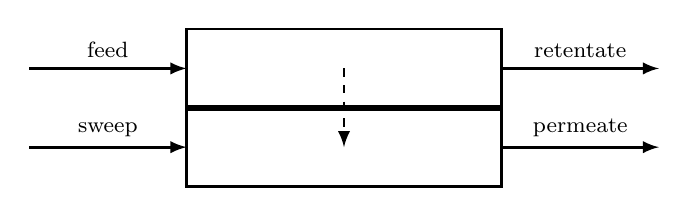
\begin{tikzpicture}[arrow/.style={line width=1pt,->,>=latex}]
	\draw [line width=1pt] (-2,2) rectangle (2,0);
	\draw [arrow] (-4,1.5) -- (-2,1.5) node [pos=0.5, above] {\footnotesize feed};
	\draw [arrow] (-4,0.5) -- (-2,0.5) node [pos=0.5, above] {\footnotesize sweep};
	\draw [arrow] (2,1.5) -- (4,1.5) node [pos=0.5, above] {\footnotesize retentate};
	\draw [arrow] (2,0.5) -- (4,0.5) node [pos=0.5, above] {\footnotesize permeate};
	\draw [line width=2pt] (-2,1) -- (2,1);
	\draw [line width=1pt,->,>=latex,dashed] (0,1.5)  -- (0,0.5) node [pos=0.5, left] {\footnotesize }; 
\end{tikzpicture}�
    	    \caption{Membrane unit for gas permeation.}
        	\label{fig:gas_permeation}
        \end{figure}

        Polymeric membranes operate at near ambient conditions. The driving force for separation is the difference
        in diffusion rates through the membrane \cite{Melin.2007}. The product flowrate and selectivity are the
        determining factors for capital cost. These are mainly dependent on the membrane area. Hence
        the capital cost for the process is expected to rise somewhat linear with the product flowrate.
        The process can economically generate a medium process stream ($\approx 20 \; t/d$) at lower purities.
        The minimal start-up time and operations near ambient conditions make the process ideal for
        applications where oxygen enriched process streams suffice and contaminants such as water or carbon
        dioxide can be tolerated. Membranes which incorporate active species that facilitate oxygen transport
        trough the membrane bear the potential to greatly improve process performance \cite{Kammermeyer.1976}.
        In general though, the alternative technologies are more mature than membrane processes.

        Processes with ion exchange membranes are drastically different from the ones with PEM's. Foremost they
        operate at high temperatures ($\approx 900 K$). At the membrane surface oxygen molecules are ionized
        and transported through the membrane along an externally applied electric potential. They travel
        through the membrane at very high flow rates. The process is capable of producing virtually pure
        oxygen. It is especially suited for integration with power generation processes \cite{Smith.2001}.

        \subsection{Hybrid processes}
        The three different alternatives presented before constitute the major technologies for separations
        of gases and therefore the production of pure nitrogen and oxygen. All technologies have their specific
        advantages and disadvantages. As the separation of gases remains a major issue when facing upcoming challenges
        for our industries substantial efforts are being made to improve current processes in terms of ecological
        and economic performance. A very promising way to achieve such improvements is to combine these technologies
        to form hybrid processes. Membranes offer many favourable characteristics are subject to limitations when
        it comes to large flow-rates and high purities. When lower purities are required or the flow-rates are limited
        they offer an efficient and cost effective way for gas separation. Therefore in the past years several
        alternatives for PSA - membrane \cite{Akinlabi.2007} or membrane-cryogenic distillation processes \cite{Wankat.2011}
        have been studied. The membrane can function within the process either as a pretreatment step, where a product enriched
        stream at medium purities and high flow-rates is produced, or after the main separation, when the main
        by-products are already removed, as a last stage to reach very high purities.

    \section{Air separation unit}
    \begin{figure}
        \footnotesize
        \center
        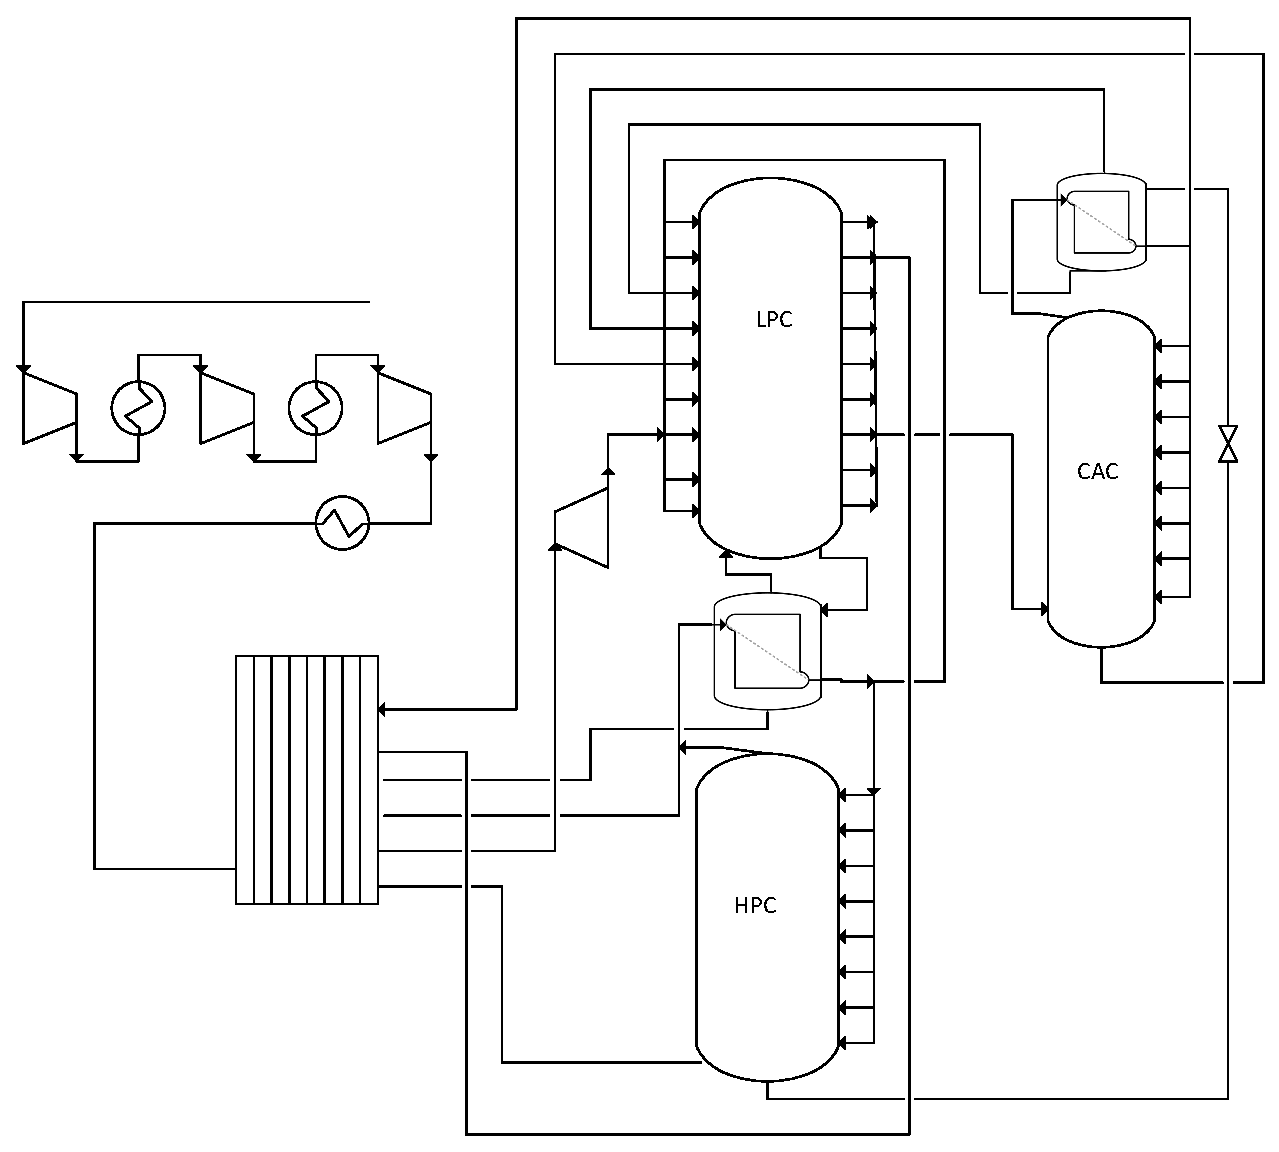
\includegraphics[width=\linewidth]{Pictures/ASU_superstructure}
        \caption{Example process superstructure.}
        \label{fig:opt:exppro}
    \end{figure}

        The developed models were combined to a process flowsheet for the cryogenic air separation process.
        As no specific process was being evaluated, the process configuration was modeled after an
        published example process flowsheet \cite{Kooijman.}. \Figref{fig:opt:exppro}
        shows the flowsheet considered henceforth. Air is drawn from the surrounding at ambient conditions
        and compressed with inter-cooling stages. Afterwards the entering process stream exchange heat
        with the product streams.

        The stream is then divided into two separate streams. One part is expanded in a turbine, and fed to
        the low pressure column (LPC) while the majority is fed to the high pressure column (HPC).
        Condenser and reboiler are combined in a single unit. A side column to the LPC generates pure
        argon. The condensate form the HPC is partially fed into the LPC. The oxygen rich sump product form the HPC
        is used to condensate the CAC top product, and afterwards fed into the LPC. From the reboiler side liquid oxygen
        is recovered from the process. From the top of LPC and HPC gaseous nitrogen is drawn. Liquid Argon is drawn from
        the CAC condenser.

        AS can be seen, this process is highly integrated with respect to energy and material streams. For both the
        steady-state and dynamic process model, the same separation sequence is considered. Compression and heat-exchange
        are only explicitly modeled in the steady-state process. While the steady-state models do provide the possibility
        to calculate pressure drops by means of an hydraulic model, they were assumed constant in all steady-state applications.
        When using the dynamic models, hydraulic equations have to be considered. For the case of the ASU process different column
        internals are often installed. The HPC as the smallest column can be economically operated as a trayed column, hence the
        respective hydraulic and cost models were employed there. The LPC and CAC are mostly equipped with structured
        packings.

        Another difference in the steady-state and dynamic models was the considered superstructure. For optimizing the number
        of separation stages, a maximum value needs to be guessed. In the steady-state case those were set to 40 for the HPC
        and 60 for the LPC and CAC respectively. With the steady-state results in mind, these were reduced to 25 for the HPC
        and 45 for LPC and CAC when constructing the dynamic process.
